\documentclass[12pt]{report}
\usepackage{graphics}
\usepackage{graphicx}
\usepackage{physics}
\usepackage{tocvsec2}
\usepackage{amsmath}
\usepackage{indentfirst}
\usepackage{epsfig}
\usepackage{fancyhdr}
\usepackage{graphicx}
\usepackage[a4paper,bindingoffset=0.2in,%
            left=1in,right=1in,top=1in,bottom=1in,%
            footskip=1cm]{geometry}
\usepackage{blindtext}
\usepackage{chngcntr}
\counterwithout{figure}{chapter}
\begin{document}
\renewcommand\bibname{References}
\pagestyle{fancy}
\fancyhead{}
\fancyfoot{}
\fancyfoot[r]{\thepage}
\fancyfoot[l]{Dept. of Computer Engineering, MEC, 2019}
\lhead{abcd}
\renewcommand{\chaptermark}[1]{
\markboth{\thechapter.\ #1}{}}
\renewcommand{\headrulewidth}{0.1pt}
\renewcommand{\footrulewidth}{0.1pt}
\fancyhead[r]{\slshape \leftmark}
\addtolength{\headheight}{\baselineskip}
\lhead{\nouppercase{\rightmark}}
\rhead{\nouppercase{\leftmark}}

\graphicspath{ {images/} }
\lhead{Deep Learning for Classical Japanese Literature}

\title {Deep Learning for Classical Japanese Literature }
\author {MDL16CS066,Kurian Benoy, kurian.bkk@gmail.com }
%\maketitle

\begin{titlepage}
\begin{center}

%\topmargin100pt
\Huge{\textbf{Deep Learning for Classical Japanese Literature}}\\
\vspace{.3in}
\large{\textbf{CS 451 Seminar}}
\vspace{1.0in}

\begin{tabbing}
xxxxxxxxxxxxxxxxxxxx\=xxxxxxxxxxxxxxxxxxxx\= xxxxxxxxxxxxxxxx\=\kill
\Large{\textbf{MDL16 CS066 }}    \>\Large{\textbf{Kurian Benoy}}\\
\end{tabbing}

\Large{\textbf{B. Tech. Computer Science \& Engineering
}}

\vspace{.6in}
\begin{figure}[h]
\begin{center}
%\epsfig{width=1in, file=embN1.jpg}
\epsfig{width=4cm, file=meclogo.png}
% If you have access to better quality logo image, that may be used,
but all the groups should use the same image
\end{center}
\end{figure}
%\vspace{.2in}
\textbf{
Department of Computer  Engineering\\
Model Engineering College Thrikkakara\\
Kochi 682021\\
Phone: +91.484.2575370\\
http://www.mec.ac.in \\ hodcs@mec.ac.in
\vspace{.1in}
}
\end{center}
\end{titlepage}

\begin{titlepage}
\begin{center}
\Large{\textbf{Model Engineering College Thrikkakara}}\\
\Large{\textbf{Dept. of Computer Engineering}}\\
\end{center}
\begin{figure}[h]
\begin{center}
\epsfig{width=4cm, file=meclogo.png}
\end{center}
\end{figure}
\begin{center}
\Large{\textbf{C E R T I F I C A T E}}\\
\vspace{.1in}
\end{center}
This is to certify that, this report titled \textbf{\textit{ Deep
Learning for Classical Japanese Literature}} is a bonafide record of
the \textbf{CS 451 Seminar} presented by
\begin{center}
 \begin{tabbing}
   xxxxxxxxxxxxxxxxxxxxxxxx\=xxxxxxxxxxxxxxxxxxxxx\=
xxxxxxxxxxxxxxxxxxxxxxxx\=\kill
\Large{\textbf{MDL16 CS066 }}     \>\Large{\textbf{Kurian Benoy}}\\
\end{tabbing}
\end{center}
\begin{center}

Seventh Semester B. Tech.
Computer Science \& Engineering  \end{center} scholar, under our
guidance and supervision, in partial
 fulfillment of the requirements for the award of the degree,\textbf{
B. Tech. Computer
Science  and Engineering} of \textbf{APJ Abdul Kalam University}.
\vspace{.2in}
\begin{tabbing}
xxxxxxxxxxxxxxxxxxxxxxxxxxxxxxxxxxxxxxxxxxxxxxxx\=
xxxxxxxxxxxxxxxxxxxxxxxxxxxxxxxx\= \kill

Guide \> Coordinator
\end{tabbing}
\begin{tabbing}
xxxxxxxxxxxxxxxxxxxxxxxxxxxxxxxxxxxxxxxxxxxxxxxx\=
xxxxxxxxxxxxxxxxxxxxxxxxxxxxxxxx\= \kill
\vspace{.1in}\\
Sreekumar K  \>Divya KB\\
Asst. Professor    \>Asst. Professor\\
Computer Engineering    \>    Computer Engineering
\end{tabbing}
\vspace{.08in}
%
\begin{tabbing}
xxxxxxxxxxxxxxxxxxxxxxxxx\= xxxxxxxxxxxxxxxxxx\= \kill
\>Head of the Department
\end{tabbing}
\begin{tabbing}
xxxxxxxxxxxxxxxxxxxxxxxxx\= xxxxxxxxxxxxxxxxxx\= \kill
\vspace{.1in}\\
%\flushleft
\today
\>Manilal D L\\
\>Associate Professor\\
\>Computer Engineering\\
\end{tabbing}
\end{titlepage}



\begin{titlepage}
\pagenumbering{roman}
%\pagebreak

\vspace{.25in}
\begin{center}
\Large{Acknowledgments}\\
\end{center}
\normalsize
\vspace{.25in}
 I would like to express my sincere gratitude to everyone who assisted
me in conducting
 this Seminar. My heartfelt gratitude to the coordinator Assistant
Professor Prof.
 Sreekumar K, Department of Computer Engineering, for giving me
permission to commence
 this seminar. I express my gratitude to Principal Prof. (Dr.) Vinu Thomas and
 Associate Professor Prof. Manilal D L, HOD of the Department of
Computer Engineering,
 Model Engineering College. Special thanks to lord, Jesus Christ for
giving me all
 energy and guidance for this endeavour.
\vspace{.25in}
\flushleft\textbf{Kurian Benoy}
\end{titlepage}


 % Abstract
\begin{abstract}
\pagenumbering{roman}

Deep Learning has given tremendous results in the past few years. With the
coming of advanced deep learning algorithms and necessary
computational resources
, Machine can outperform humans in computer vision,
can do image captioning, beat the world champion in Go.
Yet much of Deep learning research focuses on producing models which perform
well on benchmark tasks, in turn improving our understanding of the challenges
associated with those tasks. From the perspective of ML researchers,
the content of
the task itself is largely irrelevant, and thus there have increasingly been
calls for benchmark tasks to more heavily focus on problems which are of
social or cultural relevance. We are working on transforming Kuzushiji Language
to contemporary Japanese lanaguage and recognise Kuzushiji Language
which is on the
verge of extinction now. We also introduce Kuzushiji-MNIST,
a dataset which focuses on Kuzushiji (cursive Japanese), as well as two larger,
more challenging datasets, Kuzushiji-49 and Kuzushiji-Kanji.
\end{abstract}

\tableofcontents
\listoffigures

\chapter {Introduction}
\label{intro}
\pagenumbering{arabic}

\setlength{\parindent}{10ex}Japan is the land of Samurais, beautiful
Gardens, bullet
trains, Earth quakes and land of high tech technologies. Recorded
historical documents
give us a peek into the past. We are able to glimpse the world before
our time and see
its culture, norms, and values to reflect on our own. Japan has a very unique
historical pathway in that sense.

Historically, Japan and its culture was relatively isolated from the
West, until the
Meiji restoration in 1868 where Japanese leaders reformed its
education system to
modernize its culture. This caused drastic changes in the Japanese
language, writing
and printing systems.  Due to the modernization of Japanese language
in this era,
cursive Kuzhushiji is no longer taught in the official school
curriculum after a ruling
in 1900 by the Emperor.

Even though Kuzushiji had been used for over 1000 years there are very
few fluent
readers of Kuzushiji today (only 0.01 percent of modern Japanese
natives).Now Kuzushiji language is almost exsist as most of Japan
natives cannot read books written in Kuzushiji and published over 150
years ago.

In General Catalog of National Books, there are over 1.7 million books
and about 3 millions unregistered books yet to be found. It's
estimated that there are around a billion historical documents written
in Kuzhushiji language over a span of centuries. Most of this
knowledge is now inaccessible to general public. Despite ongoing
efforts to create digital copies of these documents—a safeguard
against fires, earthquakes, and tsunamis—most of the knowledge,
history, and culture contained within these texts remains inaccessible
to the general public.

While we have many digitized copies of manuscripts and books, only a
small number of people with Kuzushiji education are able to read them
and work on them, leading to a huge dataset of Japanese cultural works
which cannot be read by non-experts. To have the best for the future,
it’s always very important to preserve the current generation at its
fullest.


\chapter{Kuzushiji Dataset}
Data is known as the new oil. According to Dr Yaser S. Abu  Mustaffa
from Caltech Tech,
If someone comes to my door and tells about an interesting idea, I
will ask about the
data available. Even if the problem is not so interesting, without
data there is no
usage.

The Kuzushiji dataset is created by the National Institute of Japanese
Literature(NIJL)
and is curated by Center for Open Data in Humanities(CODH). This
dataset includes
characters in both Kanji and Hiragana, based on pre-processed images
of characters from
35 books from the 18th century. Before diving into the dataset, Let’s
understand at bit
about Japanese language.

\section{About Japanese Language}


The Japanese language can be divided into two types of systems:


\begin{itemize}
  \item \textbf{Logographic systems:}where each character represents a
word or a phrase (with thousands of characters). A prominent
logographic system is Kanji, which is based on the Chinese System.
  \item \textbf{Syllabary symbol systems:} where words are constructed
from syllables (similar to an alphabet). A prominent syllabary system
is Hiragana with 49 characters (Kuzushiji-49), which prior to the
Kuzushiji standardization had several representations for each
Hiragana character.
\end{itemize}




\section{Kuzushiji MNIST}



\begin{figure}[h]
\centering
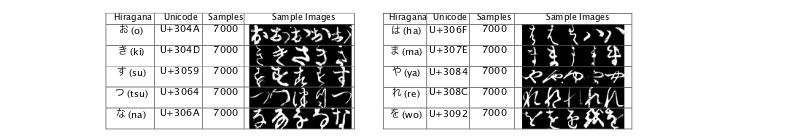
\includegraphics[width=12cm]{MNIST.png}
\caption{(a) A MNIST dataset with 5 hiranagana characters
The certain computation path is determined by a specific input applied.}
\end{figure}

MNIST dataset which is used for recognising  handwritten digits is one
of the most popular dataset's till and is usually the hello world for
Deep
Learning. As an easy to process beginner dataset, this consists of 10
classes with 7000 images for each. Yet there are fewer than 49 letters
needed to fully represent Kuzushiji Hiragana characters. So currently
we choose 10 rows of Hiragana when creating dataset with 5 letter
being stacked together to form this dataset. Each image is 28*28 pixel
resolution. Kuzhushiji MNIST is more difficult compared to MNIST
because for each image the chance for a human to detect characters
correctly when a single image is of small size and is stacked together
of 5 rows is very less.


\section{Kuzushiji-49}

Kuzushiji-49, a much larger, but imbalanced dataset containing 48
Hiragana characters and one Hiragana iteration mark with about 266,407
images.
 Both Kuzushiji-49 and Kuzushiji-MNIST consists of `grey images of
28x28 pixel resolution`. The training and test is split in ratio of
6/7 to 1/7 for each class.

\begin{figure}[h]
\centering
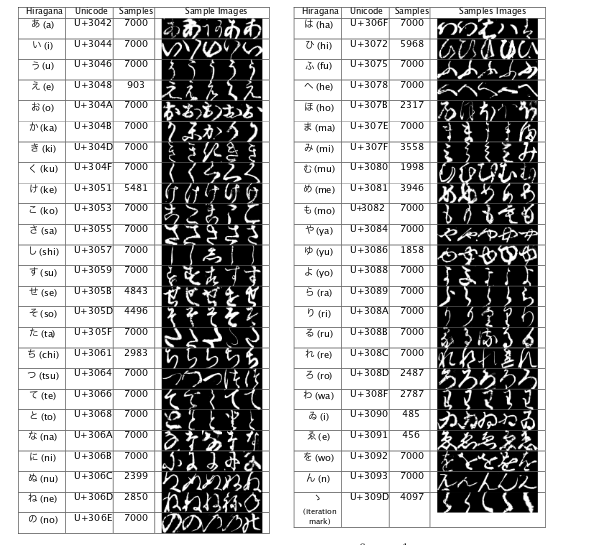
\includegraphics[width=12cm]{K49.png}
\caption{A sample of dataset of Kanji-49 with all the 48 hirangana
characters and 1 iteration mark being represented}
\end{figure}

\section{Kuzhushiji-Kanji}

Kuzushiji Kanji has a total of 3832 classes of characters  in this
dataset with about 140,426 images. Kuzushiji-Kanji images are of
larger 64x64 pixel resolution and the number of samples per class
range from over a thousand to only one sample. This dataset is not
created merely for classification images, instead for more creative
experimental task.

\begin{figure}[h]
\centering
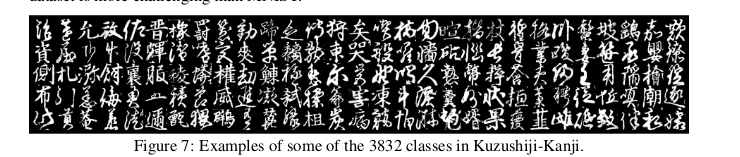
\includegraphics[width=12cm]{KK.png}
\caption{(a) The original HPC-based technique which has the malware
database and performs the analysis
locally. (b) A “sample-locally-analyze-remotely” infrastructure for
malware detection and identification. The
periodically sampled HPC values are sent to a remote server for analysis.}
\end{figure}

\section{Challenges in recognising Kuzushiji Characters}
\subsection{Large number of character types}
The total number of unique characters in the Kuzushiji dataset is over
4300. However, the frequency distribution is very long-tailed and a
large fraction of the characters (Kanji with very specific meaning)
may only appear once or twice in a book. Therefore, the dataset is
highly unbalanced.

\subsection{Hentaigana}
One characteristic of Classical Hiragana or Hentaigana (“character
variations'') is that many characters which can only be written a
single way in modern Japanese can be written in many different ways in
Kuzushiji.
For example, this image shows that Hiragana Ha (は) can be written in a
few different ways.

\begin{figure}[h]
\centering
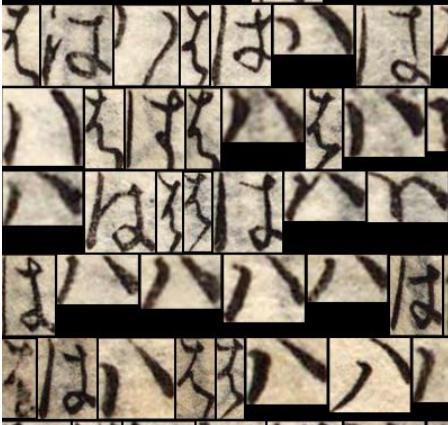
\includegraphics[width=12cm]{c1j.jpg}
\caption{ applied.}
\end{figure}

\subsection{Similarity between characters}
A few characters in Kuzushiji look very similar and it is hard to tell
what character it is without considering the above character as
context.
For example, in the image below the red circles show 3 types of
characters: Ku (く), an iteration mark and Te (て).
\begin{figure}[h]
\centering
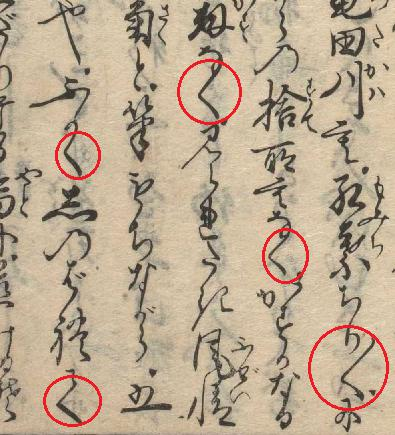
\includegraphics[width=12cm]{c2j.jpg}
\caption{(a) A MNIST dataset with 5 hiranagana characters
The certain computation path is determined by a specific input applied.}
\end{figure}

\subsection{Connectedness and overlap between characters}
Kuzushiji was written in a cursive script, and hence in many cases,
characters are connected or overlap which can make the recognition
task difficult.
In the image below, the bounding boxes in the image below show that
characters overlap. The color of the boxes are for visualization and
don’t contain any specific meaning.
\begin{figure}[h]
\centering
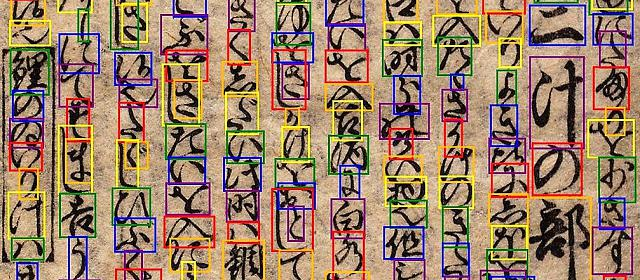
\includegraphics[width=12cm]{c3j.jpg}
\caption{(a) A MNIST dataset with 5 hiranagana characters
The certain computation path is determined by a specific input applied.}
\end{figure}

\subsection{Various Layouts}
The layout of Kuzushiji characters (while normally arranged into
columns) does not follow a single simple rule, so it is not always
trivial to express the characters as a sequence. Some examples of this
include characters being written to wrap around or even integrate into
illustrations. Sometimes, characters are written in a diagonal line.
\begin{figure}[h]
\centering
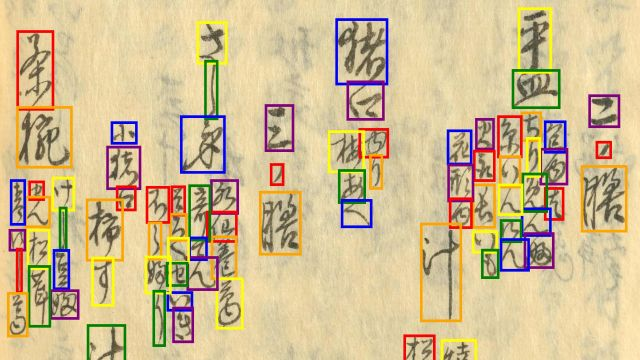
\includegraphics[width=12cm]{c4j.jpg}
\caption{(a) A MNIST dataset with 5 hiranagana characters
The certain computation path is determined by a specific input applied.}
\end{figure}

\chapter{Classification of Kuzushiji Letters}

In machine learning and statistics, classification is a supervised learning
approach in which the computer program learns from the data input
given to it and
then uses this learning to classify new observation. This data set may simply be
bi-class (like identifying whether the person is male or female or
that the mail is
spam or non-spam) or it may be multi-class too when more than two objects needs
to be classifed.

We try to focus on calculating the accuracy of recognising Kuzushiji
datasets which in both Kanji and Hiragana, based on pre-processed images of
characters from 35 books from the 18th century for datasets Kuzushiji-MNIST,
Kuzushiji-49 and Kuzushiji Kanji, each having respectively 9, 49 and
3832 classes
for the dataset.


It comes with a baseline based on the comparing with following
algorithms on Kuzushiji-MNIST and Kuzushiji-49 dataset:
\begin{enumerate}
\item four-nearest neighbours algorithm
\item 2-layer convolutional network
\item an 18-layer ResNet
\item ResNet incorporated with manifold mixup regularizer
\end{enumerate}


tt

\begin{figure}[h]
\centering
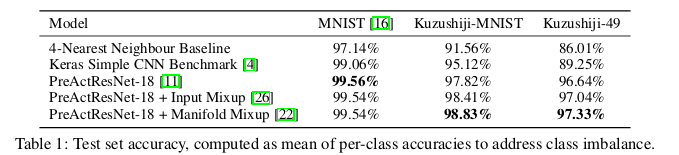
\includegraphics[width=12cm]{paperbench.png}
\caption{Fig:Test set Accuracy of various baseline models.}
\end{figure}
\\
\\
\section{Baseline Models Explained}

We have tried the following models one after the another and did
recognition of the
following Models on metric of mean-of per classes accuracy to address the class
imbalance in this model.

\subsection{ four-nearest neigbours algorithm}

The k-nearest neighbors algorithm (k-NN) is a non-parametric method used for
classification and regression. In both cases, the input consists of
the 4 closest
training examples in the feature space.

In k-NN classification, the output is a class membership. An object is
classified by a plurality vote of its neighbors, with the object being
assigned to the class most common among its k nearest neighbors (k is
a positive integer, typically small).

\subsection{2-layer convolutional network}

CNNs are regularized versions of multilayer perceptrons. Multilayer
perceptrons usually refer to fully connected networks, that is, each
neuron in one layer is connected to all neurons in the next layer. The
"fully-connectedness" of these networks makes them prone to
overfitting data. Typical ways of regularization include adding some
form of magnitude measurement of weights to the loss function.
However, CNNs take a different approach towards regularization: they
take advantage of the hierarchical pattern in data and assemble more
complex patterns using smaller and simpler patterns. Therefore, on the
scale of connectedness and complexity, CNNs are on the lower extreme.

A convolutional neural network consists of an input and an output
layer, as well as multiple hidden layers. The hidden layers of a CNN
typically consist of a series of convolutional layers that convolve
with a multiplication or other dot product. The activation function is
commonly a RELU layer, and is subsequently followed by additional
convolutions such as pooling layers, fully connected layers and
normalization layers, referred to as hidden layers because their
inputs and outputs are masked by the activation function and final
convolution. The final convolution, in turn, often involves
backpropagation in order to more accurately weight the end product

\subsection{Resnet}
Resnet is a pre-trained neural networks which was founded by Microsoft Research.
This neural networks gives state of the art result and won 1st place
in the ILSVRC 2015 classification competition with top-5 error rate of
3.57 percent
(An ensemble model). When deeper networks starts converging, a
degradation problem has been exposed: with the network depth
increasing, accuracy gets saturated and then degrades rapidly. For
almost all segmentation, classification and object
detection  and even regression with tabular data, Resnet gives state of the
art results.

\subsection{PreAct Resnet with ManiFold mixup}

A method for learning better representations, that acts as a
regularizer and despite its no significant additional computation cost
, achieves improvements over strong baselines on Supervised and
Semi-supervised Learning tasks.
 Manifold Mixup is that the dimensionality of the hidden states
exceeds the number of classes, which is often the case in practice.

\section{Resnet networks ensembled with Capsule networks}

The best results were achieved with an ensemble of VGG and ResNet – a
98.9\% accuracy on the test set, which is a state-of-the-art result on
the new dataset. TO unnderstand how this model gives this much
accuracy, it’s essential to understand about Convolutional Neural
networks. Capsule neural networks were introduced by Jeffrey Hinton
and his team to solve a very important important disadvantage of
Convolutional neural networks(CNN).

Internal data representation of a convolutional neural network does
not take into account important spatial hierarchies between simple and
complex objects. For a CNN, a mere presence of these objects can be a
very strong indicator to consider that there is a face in the image.
Orientational and relative spatial relationships between these
components are not very important to a CNN. As a mere presence of 2
eyes, a mouth and a nose in a picture does not mean there is a face,
yet CNN always see like that.

For objects in 3D representation, the relationship of various angles
and poses are not properly mapped in a usual CNN. Yet  deep learning
to better model hierarchical relationships inside of internal
knowledge representation of a neural network. Intuition behind them is
very simple and elegant. This has been now possible due to a new
algorithm for Dynamic Routing between Capsules, for calculating
distance between capsule.


On blending our architecture with Resnets which help in converging our
neural networks with less loss rate and using Capsule networks for
better representation of objects. We are able to get state of art
results for classifying Kuzushiji letters.




\chapter {Domain Transfer  Implementation}

Domain transfer focuses on pixel images, we explore instead the
transfer from pixel images to vector images, across two different
domains. Our proposed model aims to generate Modern Kanji versions of
a given Kuzushiji-Kanji input, in both pixel and stroke-based formats.
We employ KanjiVG, a font for Modern Kanji(ie the Japanese Language)
in both pixel and stroke format. This is a various interesting
application to bring life to a an almost extinct language with usage
of Machine
Learning.

\begin{figure}[h]
\centering
\includegraphics[width=12cm]{s1.png}
\caption{Kuzushiji Kanji 64x64 px samples(top) to Kanji images.}
\end{figure}

\section{Related work in Chinese Language}

There has been similar works in Chinese language to generate fake, but
plausible Chinese characters, in vector .svg format from the orginal
Kanji format of Chinese language.

We use a Generative Sequence Model framework as mentioned in Graves
paper[reference it].
To implement a  text-generation example, assuming we have a model that
has been pre-trained already, we feed in an initial random character
into the model that with an initially empty state. The model will use
the state’s information along with the current input, to generate a
probability distribution for the next character. That distribution
will be sampled randomly (possibly we distort the sampling process by
applying temperature), to obtain a prediction for the next character.
The sampled character will be placed back as the next input, as well
as the current internal state of the model.

A simple model that fits this framework is the basic N-GRAM character
modelling method. In N-GRAM, all we do is keep a record of frequencies
of the previous N characters and use the historical table of
frequencies as the probability distribution we can draw to generate
the next character.

\begin{figure}[h]
\includegraphics[scale=1]{chineGSM.png}
\caption{Generative Sequence Model Framework}
\end{figure}

This framework can also be represented by a recurrent neural network,
where the states are the hidden states of recurrent LSTM nodes, and
the output values of the network can be converted into a discrete
probability distribution via applying softmax layer to the outputs. To
train the weights of the neural network, we need a way to compare the
predicted distribution, to the actual distribution of the training
data. What is usually done is that cross-entropy loss function is
usually applied, to compare the model’s predicted probabilities after
the softmax layer, with the actual data of the entire sequence
generated.

This has been done in Graves’ sequence generation paper and
implemented as char-rnn by Karpathy. char-rnn has been used
successfully to generate not only Shakespeare’s text, but also bizarre
examples such as Linux source code, LaTeX documents, wikipedia
formatted xml articles, and music scores.

They want to model different potential states and context in the data
and be able to generate a plausible distribution of the next point
conditional to the entire historical set of points where we can then
draw from to generate our handwriting examples. Therefore in this MDN,
the inputs into the network would be the most recent relative stroke
movement, the most recent end-of-stroke signal, and the previous
hidden state of the network, while the output of the network could be
a set of values that parametrise the probability distribution of next
stroke movement and the next end-of-stroke signal.

On training the network to generate accurate distributions of the
future given the historical past, we can just sample from the
probability distribution to generate our handwriting sample. It is as
of the neural network is dreaming up some handwriting example by
feeding back to itself it’s previous generated stroke. In our demo, we
used a 2-layer stacked basic-LSTM network (no peephole connections)
with 256 nodes in each layer. Thus we are able to get fake chinese
characters which even represent new meaning while following the
correct meaning.


% Like in the inverted sinusoidal data in the previous post about
MDNs, we want to model different potential states and context in the
data and be able to generate a plausible distribution of the next
point conditional to the entire historical set of points where we can
then draw from to generate our handwriting examples. Therefore in this
MDN, the inputs into the network would be the most recent relative
stroke movement, the most recent end-of-stroke signal, and the
previous hidden state of the network, while the output of the network
could be a set of values that parametrise the probability distribution
of next stroke movement and the next end-of-stroke signal.

% Once we have trained the network to generate accurate distributions
of the future given the historical past, we can just sample from the
probability distribution to generate our handwriting sample. It is as
of the neural network is dreaming up some handwriting example by
feeding back to itself it’s previous generated stroke. In our demo, we
used a 2-layer stacked basic-LSTM network (no peephole connections)
with 256 nodes in each layer.

% Our model for the probability distribution for the future stroke
vector would be a joint 2D normal mixture distribution, charactersised
as a probabilistic weighted sum of 2D Normal distributions, each with
their own means, and covariances. We used 20 mixtures in our demo, to
be consistent with Graves’ paper, but we found actually that even 5-10
mixtures worked well enough, however the extra number of mixtures
didn’t really cause a huge drop in algorithm performance and didn’t
really increase the total size of the network, as most of the weights
were in the LSTM layers, so we just kept it at 20. If you want to
experiment with different number of nodes, node types (RNN, GRU, etc),
enable LSTM peep-hole connections, number of mixture distributions,
different DropOut probabilities – all of this can be done by setting
different flags when running train.py.

% In total, we would demand 121 output values from our network, Z,
from the MDN to infer our distribution. One of these values would be
used as the end-of-stroke probability, 20 values would define the
probability of each mixture, while the remaining 100 values constitute
20 sets of 2D Normal distribution parameters. As the output values are
real numbers that may not be bounded, we would perform a transform to
get to the values in parameter space:

% e = \frac{1}{1+ \exp(Z_{0})}


\section{Domain Transfer Architecture}
\begin{figure}[h]
\centering
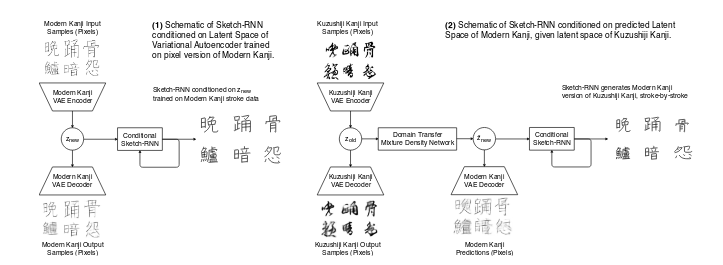
\includegraphics[scale=1]{paperdomainarch.png}
\caption{Figure: Overview of our approach (1) We first train a VAE on
pixel version of KanjiVG and Sketch-RNN model to generate stroke
version of KanjiVG conditioned on latent space Znew. (2) We train a
VAE on Kuzushiji-Kanji and train a mixture Density network to predict
P(znew|zold) and generate stroke version of Modern Kanji}
\end{figure}

Input is converted to contempary language from the old
Kuzushiji-KanjiVG format of 64x64px resolution format.
We employ KanjiVG, a font for Modern Kanji in a stroke-ordered format.
Variational Autoen-coders [14,18] provide a latent space for both
Kuzushiji-Kanji and a pixel version of KanjiVG. A Sketch-RNN  model is
then trained to generate Modern Kanji strokes, conditioned on the
VAE’slatent space. Predicting pixel versions of Modern Kanji using a
VAE also aids human transcribers as the blurry regions of the output
can be interpreted as uncertain regions to focus on.

We first train two separate ConvolutionalVariational Autoencoders, one
on the Kuzushiji-Kanji dataset, and also a second on a pixel version
ofKanjiVG dataset rendered to 64x64 pixel resolution for consistency.
The architecture for the VAEis identical to  and both datasets are
compressed into their own respective 64-dimensional latentspace,Zold
and Znew.



\subsection{Algorithm}
\begin{enumerate}
  \item Train two seperate variational autoencoder on pixel version of
KanjiVG and Kuzushiji-Kanji on 64x64px resolution.
  \item Train mixture density network to mode P(Znew | Zold) as
mixture of gaussians.
  \item Train sketch RNN to generate Kanji VGG strokes conditioned on
either znew or z~new ~P(Znew|Zold).
\end{enumerate}

\subsection{Components of this architecture}

\\
\textbf{Auto Encoders and Decoders}
\\
They are widely used unsupervised application of neural networks whose
original purpose is to find latent lower dimensional state-spaces of
datasets, but they are also capable of solving other problems, such as
image denoising, enhancement or colourization.
Variational Autoencoders is used to provide latent space of KanjiVG to
Kuzushiji Kanji. It’s used in the architecture to finetune the input
and provide better colourization and enhancement. It’s used in complex
generative models.
\\
\\
\textbf{Mixture Density Network:}
\\
Used to model density function to a new domain. It’s used for making
the neural networks to translate from Kuzushiji Kanji to KanjiVG
format in pixels.
\\
\textbf{Sketch RNN}
\\
It’s a decoder network which conditions the model in a new latent vector.

\begin{figure}[h]
\centering
\includegraphics[scale=0.4]{kurian.png}
\caption{Domain transfer process through all the components}
\end{figure}

\subsection{Comparison with Chinese architecture}
\begin{enumerate}
    \item Training two VAE encoders in our algorithm gives better
performance than single VAE encoders used.
    \item Sketch-RNN is better than char-RNN to give a better accuracy.
    \item Using adversarial losses as in other approaches is not necessary.
\end{enumerate}


\section {Why not such a system for Malayalam?}

In  Malayalam , there are about 1200+ letters in the old dravidian
Malayalam which was prominently.
In 1956 a government order reduced the total plausible characters as
120 to make it compatible with ASCII
format.

in the current Malayalam alphabets there are not much characters.
Yet there is no need for a domain transfer system in Malayalam all the Malayalam
characters are mapped in Unicode format by Swanthanthra Malayalam
community. So unlike in Japanese old and new
letter mappings in unicode format are different while in Malayalam
both have same unicode mapping.



\chapter{Conclusion}

We believe the Kuzushiji datasets will not only serve as a benchmark
to advance classificationalgorithms, but also contribute to more
creative areas such as generative modelling, adversarialexamples,
few-shot learning, transfer learning and domain adaptation. To foster
community building,we plan to organize machine learning competitions
using Kuzushiji datasets to encourage furtherdevelopment of these
research areas. We are also working on expanding the size of the
dataset, andby next year, the size of the full Kuzushiji dataset will
expand to over a million character images. We hope these efforts will
encourage further collaboration between different research fields and
at the same time, help preserve the cultural knowledge and heritage of
Japanese.

We Explored the deep learning technique for classifying Classical
Japanese, Kuzushiji and do the domain transfer to Contemporary
Japanese Language and understood the various Kuzushiji datasets





\begin{thebibliography}{999}
\addcontentsline{toc}{chapter}{References}

\bibitem{} 'Re-using Hardware Performance Counters to Detect
and Identify Kernel Control-flow Modifying
Rootkits' \\Xueyang Wang and  Ramesh Karri, IEEE Transactions on
Computer-Aided Design of Integrated Circuits and Systems
\bibitem{} 'Stealthy Malware Detection Through VMM-Based
“Out-of-the-Box” Semantic View Reconstruction' \\Xuxian Jiang, Xinyuan
Wang and Dongyan Xu , IEEE Transactions on Computer-Aided Design of
Integrated Circuits and Systems

\bibitem{}“Countering kernel rootkits
with lightweight hook protection,” in Proceedings of the 16th ACM
ConferenceZ. //Wang, X. Jiang, W. Cui, and P. Ning

\bibitem{}G. Hoglund and J. Butler, Rootkits: Subverting the windows kernel.
Boston, USA: Addison Wesley

\bibitem{} http://blog.otoro.net/2015/12/28/recurrent-net-dreams-up-fake-chinese-characters-in-vector-format-with-tensorflow/k

\bibitem{}“Kstat - kernel security therapy anti-trolls,” [Online]:
http://www.s0ftpj.
org/en/tools.html
\bibitem{}“Rkhunter,” [Online]: http://packetstormsecurity.org/files/44153/
rkhunter-1.2.8.tar.gz.html.
\bibitem{} "Graves paper Generating Sequences With Recurrent Neural
Networks" https://arxiv.org/abs/1308.0850



\end{thebibliography}
\appendix{}
\cleardoublepage
\addcontentsline{toc}{chapter}{Appendix}
\setcounter{chapter}{-1}
\addtocontents{toc}{\protect\setcounter{tocdepth}{-1}}
\chapter{Base Paper}%
https://arxiv.org/pdf/1812.01718.pdf
\end{document}

